\documentclass[11pt]{article}

\usepackage[T1]{fontenc}
\usepackage[utf8]{inputenc}
\usepackage{lmodern}
\usepackage[a4paper,margin=1in]{geometry}
\usepackage{amsmath,amssymb,amsthm,mathtools}
\usepackage{float}
\usepackage{enumitem}
\usepackage{booktabs}
\usepackage{xcolor}
\usepackage{tikz}
\usepackage{pgfplots}
\pgfplotsset{compat=1.16}
\usepackage{hyperref}
\usetikzlibrary{arrows.meta,positioning,calc,fit,backgrounds,shapes.geometric}
\usepackage{listings}
\lstset{basicstyle=\ttfamily\footnotesize,breaklines=true,columns=fullflexible,
        keepspaces=true,frame=single,framesep=4pt,xleftmargin=2pt}

\hypersetup{
    colorlinks=true,
    linkcolor=blue!70!black,
    citecolor=blue!70!black,
    urlcolor=blue!70!black
}

% ── Theorem environments ──────────────────────────────────────────────────────
\newtheorem{theorem}{Theorem}[section]
\newtheorem{proposition}[theorem]{Proposition}
\newtheorem{lemma}[theorem]{Lemma}
\newtheorem{corollary}[theorem]{Corollary}
\theoremstyle{definition}
\newtheorem{definition}[theorem]{Definition}
\newtheorem{example}[theorem]{Example}
\theoremstyle{remark}
\newtheorem{remark}[theorem]{Remark}

% ── Macros ────────────────────────────────────────────────────────────────────
\newcommand{\dist}{\operatorname{dist}}
\newcommand{\UDG}{\operatorname{UDG}}
\newcommand{\MWIS}{\mathrm{MWIS}}
\newcommand{\MIS}{\mathrm{MIS}}
\newcommand{\Efalse}{E_{\mathrm{false}}}
\newcommand{\Etrue}{E_{\mathrm{true}}}
\newcommand{\chihat}{\widehat{\chi}}
\newcommand{\R}{\mathbb{R}}
\newcommand{\N}{\mathbb{N}}
\newcommand{\indep}{\alpha}
\newcommand{\Gen}{\mathsf{Gen}}

% ── certified-reduction calculus: sorts, decoder arrow, inference-rule kit ──────
\newcommand{\tCol}{\mathsf{Col}}
\newcommand{\tIS}{\mathsf{IS}}
\newcommand{\tWIS}{\mathsf{WIS}}
\newcommand{\tUDG}{\mathsf{UDG}}
\newcommand{\tUDGa}{\widetilde{\mathsf{UDG}}}
\newcommand{\tDev}{\mathsf{Dev}}
\newcommand{\Sol}{\mathrm{Sol}}
\newcommand{\Nmax}{N_{\max}}
\newcommand{\safe}{\textsf{safe}}
\newcommand{\asafe}[1]{\textsf{asafe}(#1)}
\newcommand{\realizes}{\mathsf{realizes}}
\newcommand{\false}{\mathsf{false}}
\newcommand{\miss}{\mathsf{miss}}
\newcommand{\totopt}{\mathsf{tot\text{-}opt}}
\newcommand{\rn}[1]{\textsc{\footnotesize #1}}
\newcommand{\irule}[2]{\ensuremath{\dfrac{\;#1\;}{\;#2\;}}}
\newcommand{\redto}[1]{\mathrel{\overset{\textstyle #1}{\rightsquigarrow}}}
\newcommand{\redtos}[2]{\mathrel{\overset{\textstyle #1}{\underset{#2}{\rightsquigarrow}}}}

% ── Lightweight algorithm float (no algorithmicx dependency) ───────────────────
\newfloat{algorithm}{htbp}{loa}
\floatname{algorithm}{Algorithm}
\newcommand{\Comment}[1]{\hfill\textit{\footnotesize\textcolor{gray}{// #1}}}

% ─────────────────────────────────────────────────────────────────────────────
\title{%
  \textbf{Certified Compilation of Graph Coloring to Neutral-Atom Hardware}\\[0.45em]
  \large An Exact Gadgetized Reduction with a Heuristic Layout Optimizer}
\author{Research Draft}
\date{\today}

\begin{document}
\maketitle

\begin{abstract}
Neutral-atom quantum processors solve a single native problem---maximum-weight
independent set (MWIS) on a unit-disk graph (UDG)---and do not color graphs, so any
coloring pipeline must \emph{reduce} coloring to UDG--MWIS rather than embed the
input geometrically. We present such a pipeline: an exact, polynomial-time two-stage
reduction (colorability to independent set on an auxiliary graph of size $nk$, then
a Nguyen-style gadgetization into a weighted UDG) whose correctness is a once-proved,
inflation-free meta-theorem with an exact decoder, leaving only geometry---atom
count, area, crossings, analog-solve quality---as engineering risk; a provable
impossibility result demotes the natural geometric-supergraph alternative to a
correctness-neutral layout optimizer. We cast the whole pipeline as a
\emph{coloring-specification language} with a \emph{certified-reduction type system}
whose types are problem reductions carrying executable decoders, so end-to-end
soundness and the legal stage order follow from typing, and we back this with an
axiom-free Coq mechanization, a Haskell type checker, and a faithful Rydberg
simulator. Empirically the reduction matches a brute-force oracle on $18/18$ named
instances, a certified separator decomposition breaks the $2^{nk}$ simulation wall
(every device solve $\le 13$ atoms while the whole-instance $nk$ reaches $192$), and
the pipeline certifies the chromatic number exactly on the DIMACS Mycielski
benchmark in both directions.
\end{abstract}

\paragraph{Keywords.} graph coloring, unit-disk graphs, maximum independent set,
Rydberg blockade, neutral-atom computing, gadget reductions, certified
compilation, QuEra, Bloqade.

% =============================================================================
\section{Introduction}
\label{sec:intro}
% =============================================================================

Graph coloring is a canonical NP-complete problem~\cite{Karp1972,GareyJohnson1979}
with broad practical reach, from register allocation and scheduling to frequency
assignment. A recent and physically distinctive way to attack such combinatorial
problems is the neutral-atom quantum platform, in which individually trapped atoms
are excited to Rydberg states and interact through the \emph{Rydberg
blockade}~\cite{Saffman2010,Henriet2021,Scholl2022}. The decisive feature of this
platform is geometric: two atoms within a blockade radius $r$ cannot both be
excited, so the set of simultaneously excited atoms is precisely an
\emph{independent set} of the unit-disk graph (UDG) induced by atom positions.
The device's analog ground state therefore encodes a \emph{maximum-weight
independent set} (MWIS) of that UDG~\cite{Pichler2018,Ebadi2022}.

This single fact frames the entire compilation problem and is the pivot of this
paper:

\begin{quote}
\itshape
The hardware solves MWIS on a unit-disk graph. It does not color. Any pipeline
that compiles coloring to this hardware must \emph{reduce} coloring to UDG--MWIS,
not merely \emph{embed} the input graph geometrically.
\end{quote}

There are two natural strategies for getting an arbitrary coloring instance onto
this hardware, and the distinction between them organizes the whole paper.

\paragraph{Design A --- geometric supergraph embedding.} Place the original
vertices in $\R^2$ and choose a radius $r$ so that the induced UDG $H$ is a
\emph{supergraph} of the input $G$, i.e.\ $E(G)\subseteq E(H)$. Then any proper
coloring of $H$ restricts to a proper coloring of $G$. This is attractive because
the supergraph relation is trivially achievable and gives a one-line decoder.
Section~\ref{sec:heuristics} develops the seven heuristics that make $H$ as good
as possible. However, Design A has two structural defects. First, we prove
(Theorem~\ref{thm:impossibility}) that a same-vertex UDG supergraph
\emph{cannot} bound chromatic-number inflation in general: the star $K_{1,n}$ has
$\chi = 2$ but forces $\chi(H)\ge\lceil n/5\rceil\to\infty$ in any UDG supergraph.
Second, and independently, even a perfect $H$ is not executable, because the
device cannot color $H$; coloring a UDG on an MWIS machine requires iterated
independent-set extraction, which is itself heuristic. Design A is thus heuristic
twice and unbounded once.

\paragraph{Design B --- exact gadgetized reduction.} Reduce $k$-colorability of
$G$ to a \emph{single} MWIS instance, then embed that instance into a weighted UDG
the hardware can run. This is the standard reduction route, and it composes two
exact, polynomial-time steps (Section~\ref{sec:gadget}): the classical
colorability$\to$independent-set reduction, and the Rydberg gadgetization of an
arbitrary graph into a UDG via copy/crossing gadgets~\cite{Nguyen2023}. Here
correctness is a once-proved meta-theorem with no inflation and an exact inverse
decoder. The remaining uncertainty is not about \emph{whether} the answer is
correct but about \emph{whether it fits the device and whether the analog
dynamics finds the ground state} --- both geometric/physical questions.

We adopt Design B as the primary path and retain Design A's heuristics in a
strictly subordinate, and now sound, role: the \emph{layout optimizer} that
realizes the gadgetized instance under hardware spacing while minimizing atom
count, area, and crossings. Because the gadget structure is fixed and exact, the
heuristics can no longer affect correctness --- only feasibility and solve
quality. This relocation is the central design decision of the paper.

\paragraph{Contributions.} In summary, this paper contributes:
\begin{enumerate}[label=(\arabic*),leftmargin=2.2em]
  \item A clean statement of the compilation problem that takes the hardware's
        native primitive (UDG--MWIS) as the target, and a two-layer pipeline that
        separates exact correctness from heuristic geometry
        (Sections~\ref{sec:overview}--\ref{sec:gadget}).
  \item The exact primary reduction: colorability$\to$MIS with a self-contained
        correctness proof and size $nk$ (Theorem~\ref{thm:col2is}), composed with
        Rydberg UDG gadgetization (Theorem~\ref{thm:gadget}) to give an end-to-end
        exactness and decoding meta-theorem (Theorem~\ref{thm:endtoend}), together
        with $O((nk)^2)$ atom-count and feasibility bounds
        (Section~\ref{sec:size}).
  \item An impossibility result (Theorem~\ref{thm:impossibility}) that rigorously
        explains why the geometric-supergraph approach cannot be the correctness
        mechanism, justifying its demotion.
  \item Seven polynomial-time geometric heuristics, corrected and re-targeted as a
        hardware-aware \emph{layout optimizer} for the gadget instance, with
        termination guarantees and a corrected catalogue of provably exact graph
        families (Section~\ref{sec:heuristics}).
  \item An integrated pipeline with worked examples and a full complexity
        accounting (Sections~\ref{sec:pipeline}--\ref{sec:complexity}).
  \item A coloring-specification \emph{language} and a \emph{certified-reduction
        type system} (Section~\ref{sec:lang}): problem-type sorts indexed by the
        invariants the reductions preserve, a single decoder-carrying reduction
        judgment, per-stage typing rules whose composition is the soundness theorem
        (Theorem~\ref{thm:typesound}), a corollary that the legal stage order is
        forced by typing (Corollary~\ref{cor:order}), and refinements for
        certificate grade, the impossibility-gated supergraph safety effect, and
        bounded-width decomposition.
  \item A working implementation and a quantitative evaluation
        (Section~\ref{sec:eval}): (a) an \emph{axiom-free} Coq/Rocq mechanization
        of the certified-reduction calculus, so Stage-1 exactness, the gadget
        offset invariant, end-to-end pipeline soundness, and the legal stage
        ordering are machine-checked theorems; (b) a prototype typed front end in
        Haskell (parser, type-and-effect checker, elaborator, device emitter)
        passing $12{,}230$ test checks; and (c) an empirical validation against a
        brute-force oracle and a faithful Rydberg adiabatic simulator, including a
        certified separator decomposition that defeats the $2^{nk}$ classical-
        simulation wall and a run of the canonical DIMACS Mycielski benchmark on
        which the chromatic number is certified exactly.
\end{enumerate}

\paragraph{Structure of the paper.} Section~\ref{sec:related} reviews related work
on coloring, unit-disk graphs, Rydberg MWIS reductions, graph decomposition, and
type-and-effect systems. Section~\ref{sec:overview} sets up the problem and the
two-layer pipeline. Section~\ref{sec:gadget} develops the exact primary path---the
two reductions, their end-to-end correctness, the size and feasibility bounds, and a
worked example. Section~\ref{sec:heuristics} proves the impossibility result for the
geometric-supergraph approach and re-targets the seven heuristics as a layout
optimizer. Section~\ref{sec:pipeline} assembles the integrated pipeline and
Section~\ref{sec:complexity} gives its complexity. Section~\ref{sec:lang} presents
the coloring-specification language and the certified-reduction type system, and
Section~\ref{sec:eval} reports the Coq mechanization, the Haskell implementation, and
the empirical validation. Sections~\ref{sec:discussion} and~\ref{sec:future} discuss
limitations and future work, and Section~\ref{sec:conclusion} concludes.

% =============================================================================
\section{Related Work}
\label{sec:related}
% =============================================================================

\paragraph{Graph coloring and its complexity.} Deciding $k$-colorability for
$k\ge 3$ is NP-complete~\cite{Karp1972,GareyJohnson1979}, and the chromatic number
is hard even to approximate. The chromatic number has been studied through the
chromatic polynomial since Tutte~\cite{Tutte1954}, and deep lower bounds come from
topological methods such as Lov\'asz's resolution of the Kneser
conjecture~\cite{Lovasz1983}; our benchmark family, the Mycielskians
(Section~\ref{sec:dimacs}), is the standard source of triangle-free graphs with
arbitrarily large $\chi$. Practical colorings are produced by greedy orderings
such as largest-first~\cite{Welsh1967} and by the saturation-degree heuristic
DSATUR~\cite{Brelaz1979}; the clique number gives the basic lower bound
$\omega(G)\le\chi(G)$~\cite{West2001}, and computing it is itself the (NP-hard)
maximum-clique problem~\cite{Bomze1999}. We use DSATUR only as an auxiliary
\emph{witness} generator in the secondary path, never on the exact path.

\paragraph{Unit-disk graphs.} UDGs are the intersection graphs of unit disks in
the plane~\cite{Clark1990UDG}. Recognition --- deciding whether a given abstract
graph is a UDG --- is NP-hard~\cite{Breu1998,Jungck2021}, which is precisely why
we never attempt exact realization of the input graph. The geometric constraint
interacts sharply with coloring: even unit-\emph{distance} graphs in the plane can
already force $\chi=4$~\cite{Clark1990}, underscoring that distance-based
adjacency carries genuine chromatic content. UDGs enjoy strong
geometric locality: every clique lies inside a disk of radius $r$, and the
packing of points in such a disk is bounded~\cite{Heppes2003}, a fact we use both
for the impossibility result and for clique control.

\paragraph{Rydberg MWIS and gadgetized reductions.} The identification of the
Rydberg blockade ground state with MWIS on a UDG is due to
Pichler et al.~\cite{Pichler2018} and was demonstrated at scale on hundreds of
atoms by Ebadi et al.~\cite{Ebadi2022}. Because native UDGs are geometrically
restricted, Nguyen et al.~\cite{Nguyen2023} introduced copy and crossing gadgets
that encode MWIS on an \emph{arbitrary} graph as MWIS on a weighted UDG laid out
on a grid, with a known value offset and a structural decoder. Our primary path
is exactly the composition of the classical colorability$\to$MIS reduction with
this gadgetization; the hardware target is QuEra's neutral-atom
machine~\cite{Wurtz2023}, programmed through the Bloqade simulation stack. The
programmable-Rydberg platform has matured rapidly---from quantum phases in optical
lattices~\cite{Ebadi2021} to multi-qubit gate-model
processors~\cite{Graham2022}---and competing quantum hardware such as photonic
systems~\cite{Madsen2023} targets the same optimization problems by different
physical means; our compilation strategy is, however, specific to the UDG--MWIS
primitive of the Rydberg blockade. Variational
and analog quantum optimization more broadly is surveyed
in~\cite{Cerezo2021,Preskill2018}.

\paragraph{Spectral and force-directed layout.} Our layout optimizer draws on
classical embedding machinery: the graph Laplacian and its
eigenvectors~\cite{Chung1997,Fiedler1973}, Laplacian
eigenmaps~\cite{Belkin2003}, force-directed drawing~\cite{Fruchterman1991},
multidimensional scaling~\cite{Kruskal1964}, and
gradient-based optimization~\cite{Nesterov2004,Boyd2004}. Where the smooth
objective is inadequate---e.g.\ escaping the discrete penalty landscape of
false-edge repair---the same role can be played by combinatorial metaheuristics
such as simulated annealing~\cite{Kirkpatrick1983} or tabu
search~\cite{Glover1997}. These are standard
tools; our contribution is not the tools but their re-targeting to a
\emph{correctness-neutral} role behind an exact reduction.

\paragraph{Graph decomposition and bounded width.} Our scaling layer
(Section~\ref{sec:decomp}) rests on classical structure theory. Chordal (rigid-
circuit) graphs always admit clique separators~\cite{Dirac1961}, and Tarjan's
clique-separator decomposition~\cite{Tarjan1985} turns such separators into a
divide-and-conquer schedule---exactly the case in which our \rn{Stitch} rule needs
no boundary search. More generally, tree-width and the graph-minors
program~\cite{RobertsonSeymour1986} explain why many NP-hard problems, coloring
among them, become tractable on bounded-width
instances~\cite{ArnborgProskurowski1989}, with linear-time tree-decomposition
available for fixed width~\cite{Bodlaender1996}. The separator search, connected-
component analysis, and boundary bookkeeping in our decomposition driver are
textbook graph algorithms~\cite{Cormen2009}. Our contribution is to make the
width-bounded device budget $(wk)^2\le\Nmax$ a \emph{typed} premise
(Section~\ref{sec:refine}) rather than an after-the-fact analysis.

\paragraph{Type-and-effect systems.} The certified-reduction calculus of
Section~\ref{sec:lang} follows the broader line of work on type-and-effect systems
for static analysis pioneered by Lucassen and Gifford's polymorphic effect
systems~\cite{LucassenGifford1988} and subsequently extended by Ferrari and
collaborators to resource-usage policies, behavioural analyses, and security
properties~\cite{BodeiDeganoFerrari1998,BartolettiDeganoFerrariZunino2009,DeganoFerrariGalletta2016}.
In contrast to conventional effects that approximate program execution, our effects
represent \emph{guarantees about answer-preserving reductions and chromatic-number
inflation bounds}---the safety effect tracks whether a transform preserves or
boundedly inflates $\chi$ and accumulates the bound through a monoid, gated by the
geometric impossibility theorem. This shows that the same static-analysis paradigm
can be lifted from program properties to optimization-problem transformations.

% =============================================================================
\section{Problem Setup and Pipeline Overview}
\label{sec:overview}
% =============================================================================

We consider finite simple undirected graphs $G=(V,E)$ with $n=|V|$, $m=|E|$.

\begin{definition}[Proper $k$-coloring; chromatic number]
A proper $k$-coloring is a map $c:V\to\{1,\dots,k\}$ with $c(u)\ne c(v)$ for every
$\{u,v\}\in E$. The chromatic number $\chi(G)$ is the least $k$ admitting one.
\end{definition}

\begin{definition}[Unit-disk graph]
Given a placement $p:V\to\R^2$ and radius $r>0$, the induced UDG $\UDG(p,r)$ has an
edge $\{u,v\}$ iff $\|p(u)-p(v)\|_2\le r$. A weighted UDG additionally assigns a
weight $w:V\to\R_{>0}$.
\end{definition}

\begin{definition}[Independent set; MWIS]
An independent set of $H$ is a vertex set with no internal edge. For weights $w$,
the maximum-weight independent set value is
$\MWIS(H,w)=\max\{\sum_{v\in S}w(v):S\text{ independent}\}$. For unit weights this
is the independence number $\indep(H)$.
\end{definition}

\paragraph{Hardware primitive.} A neutral-atom array with atoms at positions
$p(v)$ and blockade radius $r$ realizes $\UDG(p,r)$; under appropriate driving its
many-body ground state encodes $\MWIS(\UDG(p,r),w)$, where $w$ is set by local
detunings~\cite{Pichler2018,Ebadi2022}. The device constraints are a minimum atom
spacing $d_{\min}$, a maximum blockade radius $r_{\max}$, a finite array area
$A_{\max}$, and a maximum atom count $N_{\max}$~\cite{Wurtz2023}.

\paragraph{The two-layer pipeline.} Figure~\ref{fig:overview} shows the design.
The primary (exact) path reduces coloring to an \emph{abstract} weighted UDG--MWIS
instance and decodes the measured independent set back to a coloring. The
secondary (heuristic) path is the geometric engine that turns the abstract gadget
instance into concrete atom coordinates obeying the hardware constraints, and is
also available as a stand-alone --- but only chromatic-non-decreasing --- coloring
backend for comparison.

\begin{figure}[h]
\centering
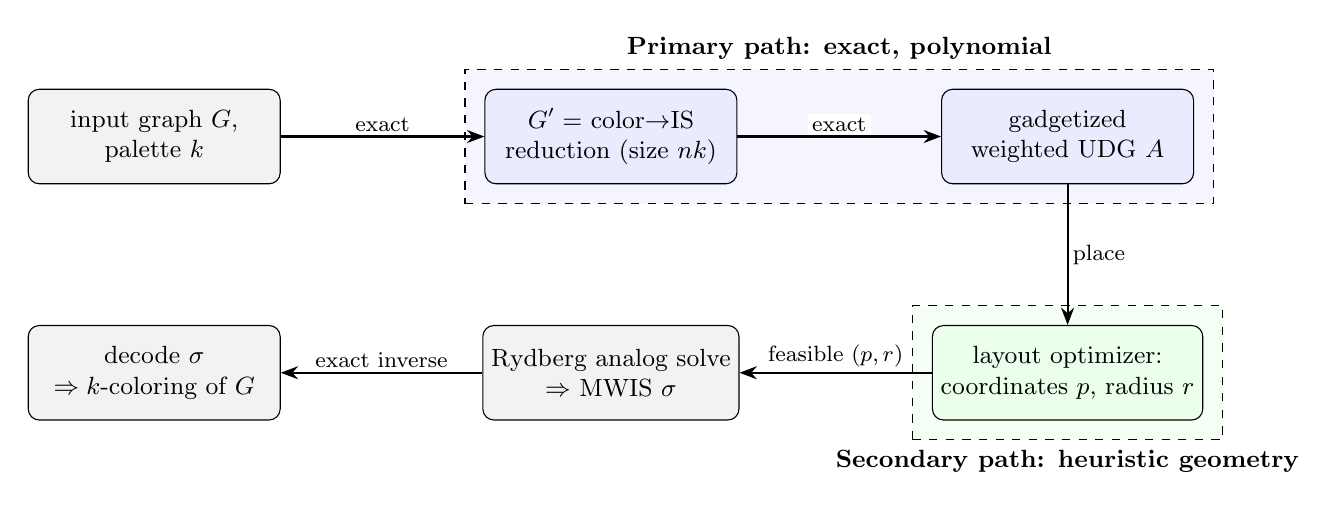
\begin{tikzpicture}[
  font=\small,
  box/.style={rectangle,draw,rounded corners,minimum width=32mm,minimum height=12mm,align=center,inner sep=3pt},
  exact/.style={box,fill=blue!8},
  heur/.style={box,fill=green!8},
  io/.style={box,fill=gray!10},
  ar/.style={-{Stealth[length=2.2mm]},thick},
  lbl/.style={font=\footnotesize,fill=white,inner sep=1.5pt}
]
% top row (left to right)
\node[io]    (G)  at (0,0)     {input graph $G$,\\ palette $k$};
\node[exact] (Gp) at (5.8,0)   {$G'=$ color$\to$IS\\ reduction (size $nk$)};
\node[exact] (A)  at (11.6,0)  {gadgetized\\ weighted UDG $A$};
% bottom row (right to left)
\node[heur]  (layout) at (11.6,-3) {layout optimizer:\\ coordinates $p$, radius $r$};
\node[io]    (solve)  at (5.8,-3)  {Rydberg analog solve\\ $\Rightarrow$ MWIS $\sigma$};
\node[io]    (dec)    at (0,-3)    {decode $\sigma$\\ $\Rightarrow k$-coloring of $G$};

\draw[ar] (G)  -- node[lbl,above]{exact} (Gp);
\draw[ar] (Gp) -- node[lbl,above]{exact} (A);
\draw[ar] (A)  -- node[lbl,right]{place} (layout);
\draw[ar] (layout) -- node[lbl,above]{feasible $(p,r)$} (solve);
\draw[ar] (solve)  -- node[lbl,above]{exact inverse} (dec);

\begin{scope}[on background layer]
  \node[draw,dashed,fill=blue!4,fit=(Gp)(A),inner sep=7pt,
        label=above:{\textbf{Primary path: exact, polynomial}}] {};
  \node[draw,dashed,fill=green!4,fit=(layout),inner sep=7pt,
        label=below:{\textbf{Secondary path: heuristic geometry}}] {};
\end{scope}
\end{tikzpicture}
\caption{The two-layer pipeline. Correctness lives entirely in the blue (exact)
path; the green (heuristic) path determines only hardware feasibility and
analog-solve quality.}
\label{fig:overview}
\end{figure}

% =============================================================================
\section{Primary Path: Exact Gadgetized Reduction}
\label{sec:gadget}
% =============================================================================

The primary path is the composition of two exact reductions:
\[
  \underbrace{G,k}_{\text{coloring}}
  \;\xrightarrow{\;\text{Stage 1}\;}\;
  \underbrace{G'}_{\text{MIS instance, size }nk}
  \;\xrightarrow{\;\text{Stage 2}\;}\;
  \underbrace{A=(\,p,r,w\,)}_{\text{weighted UDG}}
  \;\xrightarrow{\;\text{solve}\;}\;
  \sigma
  \;\xrightarrow{\;\text{decode}\;}\;
  \text{coloring of }G.
\]

\subsection{Stage 1: Colorability $\to$ Independent Set}
\label{sec:col2is}

\begin{definition}[Color-choice graph]
\label{def:choice}
Given $G=(V,E)$ and palette size $k$, the \emph{color-choice graph}
$G'=(V',E')$ has vertex set $V'=V\times\{1,\dots,k\}$, and edge set $E'=E'_{\mathrm{choice}}\cup E'_{\mathrm{conflict}}$ where
\begin{align*}
  E'_{\mathrm{choice}}   &= \bigl\{\{(v,i),(v,j)\} : v\in V,\ 1\le i<j\le k\bigr\},
   &&\text{(a $k$-clique per vertex)}\\
  E'_{\mathrm{conflict}} &= \bigl\{\{(u,i),(v,i)\} : \{u,v\}\in E,\ 1\le i\le k\bigr\}.
   &&\text{(same-color conflicts)}
\end{align*}
All vertices carry unit weight. Then $|V'|=nk$ and
$|E'|=n\binom{k}{2}+mk$.
\end{definition}

The choice-clique enforces ``at most one color per vertex''; the conflict edges
enforce ``adjacent vertices differ in color.''

\begin{theorem}[Exactness of Stage 1]
\label{thm:col2is}
For every graph $G$ and every $k\ge 1$,
\[
  \indep(G') = n \quad\Longleftrightarrow\quad G \text{ is } k\text{-colorable},
\]
and $\indep(G')\le n$ always. Moreover, independent sets of $G'$ of size $n$ are in
explicit bijection with proper $k$-colorings of $G$.
\end{theorem}

\begin{proof}
For each $v$, the $k$ vertices $\{(v,i)\}_i$ form a clique
($E'_{\mathrm{choice}}$), so any independent set $S$ contains at most one slot per
original vertex; hence $|S|\le n$.

($\Leftarrow$) Let $c$ be a proper $k$-coloring. Put
$S=\{(v,c(v)):v\in V\}$, so $|S|=n$. $S$ is independent: it has exactly one slot
per vertex (no choice edge is internal), and for any $\{u,v\}\in E$ we have
$c(u)\ne c(v)$, so no conflict edge $\{(u,c(u)),(v,c(v))\}$ exists --- conflict
edges only join \emph{equal} color indices. Thus $\indep(G')\ge n$, and combined
with $\indep(G')\le n$ we get $\indep(G')=n$.

($\Rightarrow$) Let $S$ be independent with $|S|=n$. By the choice-clique bound $S$
has exactly one slot per vertex, defining $c(v)=i$ where $(v,i)\in S$. For
$\{u,v\}\in E$, if $c(u)=c(v)=i$ then $\{(u,i),(v,i)\}\in E'_{\mathrm{conflict}}$
would be internal to $S$, contradicting independence. Hence $c$ is proper.

The two maps $c\mapsto S$ and $S\mapsto c$ are mutually inverse, giving the
bijection.
\end{proof}

\begin{remark}[Fixed-$k$ vs.\ chromatic number]
A single value $k$ tests $k$-colorability. The chromatic number is obtained by a
sweep: the least $k$ with $\indep(G')=n$ equals $\chi(G)$. Binary search over
$k\in\{1,\dots,n\}$ costs $O(\log n)$ solves.
\end{remark}

\subsection{Stage 2: Independent Set $\to$ Unit-Disk MWIS}
\label{sec:gadgetize}

$G'$ is an abstract graph and is generally not a UDG. Stage 2 embeds it into a
weighted UDG that the hardware can realize, using the copy/crossing gadget
construction of Nguyen et al.~\cite{Nguyen2023}, itself building on the Rydberg
MWIS encoding of Pichler et al.~\cite{Pichler2018}. We use it as a black box with
a precise interface.

\begin{theorem}[Gadgetized UD-MWIS embedding~\cite{Nguyen2023}]
\label{thm:gadget}
There is a polynomial-time procedure $\mathsf{gadgetize}$ that maps any vertex-weighted
graph $G'=(V',E',w')$ to a weighted unit-disk graph $A=(p,r,w)$ on a grid, together
with a designated set of \emph{logical} atoms $\ell:V'\hookrightarrow V(A)$ and a
constant $C\ge 0$, such that
\[
  \MWIS(A,w) = \MWIS(G',w') + C,
\]
and every maximum-weight independent set $S_A$ of $A$ restricts on the logical
atoms to a maximum-weight independent set $\sigma=\ell^{-1}(S_A\cap \ell(V'))$ of
$G'$. The number of atoms is $|V(A)| = O\!\left(|V'|^2\right)$ in the worst case,
governed by the number of edge crossings in the chosen planar layout of $G'$.
\end{theorem}

The construction places the $|V'|$ logical atoms along a diagonal and routes each
edge of $G'$ as a chain of \emph{copy} gadgets that propagate an atom's
occupation; wherever two routed edges must cross, a \emph{crossing} gadget passes
both signals through without spurious coupling. Weights are chosen so that the
ground-state independent set selects logical atoms exactly according to a maximum
independent set of $G'$. We treat the exact gadget weights as fixed by
\cite{Nguyen2023}; choosing or re-deriving a custom gadget set is an engineering
fork (Section~\ref{sec:future}).

\subsection{Decoding and End-to-End Correctness}
\label{sec:decode}

Decoding composes the two inverses. Given a hardware-measured independent set
$S_A$ of $A$: (1) restrict to logical atoms and apply $\ell^{-1}$ to obtain
$\sigma\subseteq V'$ (Stage-2 inverse); (2) if $|\sigma|=n$, read the coloring
$c(v)=i$ for the unique $(v,i)\in\sigma$ (Stage-1 inverse). The full chain is the
following meta-theorem, proved once for all instances.

\begin{theorem}[End-to-end exactness]
\label{thm:endtoend}
Let $A=\mathsf{gadgetize}(G')$ for $G'$ the color-choice graph of $(G,k)$. Then:
\begin{enumerate}[label=(\roman*),leftmargin=2.2em]
  \item $\MWIS(A,w) = n + C$ if and only if $G$ is $k$-colorable.
  \item Any maximum-weight independent set of $A$ with logical-atom weight $n$
        decodes, via $\ell^{-1}$ followed by the Stage-1 readout, to a proper
        $k$-coloring of $G$.
  \item The construction and the decoder both run in time polynomial in $n$ and
        $k$, and the decoder is an exact inverse of the construction --- there is
        no chromatic-number inflation.
\end{enumerate}
\end{theorem}

\begin{proof}
By Theorem~\ref{thm:gadget}, $\MWIS(A,w)=\MWIS(G',w')+C=\indep(G')+C$ (unit
weights). By Theorem~\ref{thm:col2is}, $\indep(G')=n$ iff $G$ is $k$-colorable, and
$\indep(G')\le n$ always; this gives (i). For (ii), a maximum independent set of
$A$ restricts (Theorem~\ref{thm:gadget}) to a maximum independent set $\sigma$ of
$G'$; when its size is $n$, the Stage-1 bijection (Theorem~\ref{thm:col2is}) reads
$\sigma$ off as a proper coloring. Polynomiality in (iii) is immediate: Stage 1 is
$O(nk+mk)$ to build, Stage 2 is polynomial by Theorem~\ref{thm:gadget}, and both
readouts are linear in their outputs. Exactness of each inverse was established in
the respective theorems, and exactness composes.
\end{proof}

\begin{remark}[Where uncertainty actually lives]
Theorem~\ref{thm:endtoend} is unconditional: it never assumes the analog solve
succeeds. The two real risks are (a) \emph{feasibility} --- whether $A$ fits inside
$N_{\max}$ atoms and $A_{\max}$ area (Section~\ref{sec:size}), and (b)
\emph{analog-solve quality} --- whether the Rydberg dynamics reaches the MWIS
ground state rather than a low-lying excited state. Neither is a correctness
question about the reduction, and a returned independent set is always
\emph{verifiable}: $|\sigma|=n$ certifies a valid coloring, $|\sigma|<n$ certifies
only that the solver did not find a witness.
\end{remark}

\subsection{Size and Feasibility Bounds}
\label{sec:size}

\begin{proposition}[Atom budget]
\label{prop:atombudget}
For an instance $(G,k)$ with $|V|=n$, the gadgetized UDG $A$ uses
\[
  |V(A)| = O\!\bigl((nk)^2\bigr)
\]
atoms in the worst case, and at least $nk$ (the logical atoms). The instance is
hardware-feasible only if $|V(A)|\le N_{\max}$ and the layout fits within
$A_{\max}$ under spacing $d_{\min}$.
\end{proposition}

\begin{proof}
Stage 1 produces $|V'|=nk$ logical vertices; Stage 2 contributes
$O(|V'|^2)$ atoms by Theorem~\ref{thm:gadget}. The lower bound is the logical-atom
count.
\end{proof}

The quadratic blow-up against a few-hundred-atom device~\cite{Wurtz2023} is the
practical bottleneck, and it is exactly what the layout optimizer of
Section~\ref{sec:heuristics} attacks. Two preprocessing knobs reduce the effective
size before gadgetization:
\begin{itemize}[leftmargin=1.4em]
  \item \textbf{Graph simplification.} Removing vertices of degree $<k$ (they are
        always colorable last), contracting degree-2 chains, and decomposing on
        cut vertices and biconnected components all shrink $n$ without changing
        $k$-colorability.
  \item \textbf{Crossing minimization.} Because Stage 2's atom count is dominated
        by edge crossings, a good planar-ish layout of $G'$ (or of $G$ before
        expansion) directly lowers $|V(A)|$. This is a geometric objective --- the
        province of the heuristics.
\end{itemize}

\subsection{Worked Example: $3$-Coloring a Small Graph}
\label{sec:gadget-example}

\begin{example}
Let $G$ be the $4$-cycle $C_4$ with vertices $v_1v_2v_3v_4$ and $k=3$. Stage 1
builds $G'$ on $V'=\{(v_a,i): a\in\{1,2,3,4\},\,i\in\{1,2,3\}\}$, $|V'|=12$. Each
vertex contributes a choice-triangle on its three slots; each edge of $C_4$
contributes three conflict edges (one per color). A proper $3$-coloring such as
$c=(1,2,1,2)$ corresponds to the independent set
$\{(v_1,1),(v_2,2),(v_3,1),(v_4,2)\}$ of size $4=n$, and conversely. Since
$\chi(C_4)=2\le 3$, Stage 1 reports $\indep(G')=4$, so $G$ is $3$-colorable.
Gadgetizing $G'$ yields a weighted UDG with $12$ logical atoms plus routing/crossing
atoms; measuring its MWIS and applying $\ell^{-1}$ recovers the size-$4$ set, whose
Stage-1 readout is the coloring $(1,2,1,2)$. No inflation occurs at any step.
\end{example}

% =============================================================================
\section{Secondary Path: Heuristic Geometry and the Layout Optimizer}
\label{sec:heuristics}
% =============================================================================

We now develop the geometric heuristics. We first prove why they cannot serve as
the coloring-correctness mechanism, then state the role they actually play.

\subsection{Why Geometric Supergraphs Cannot Bound Inflation}
\label{sec:impossibility}

\begin{definition}[Safe supergraph; color inflation]
A UDG $H=\UDG(p,r)$ on the same vertex set $V$ as $G$ is a \emph{safe supergraph}
if $E(G)\subseteq E(H)$. The \emph{false edges} are $\Efalse=E(H)\setminus E(G)$,
and the \emph{color-inflation ratio} is $\rho = \chihat(H)/\chihat(G)$, where
$\chihat$ is a chromatic estimate (e.g.\ DSATUR).
\end{definition}

\begin{proposition}[Safety $\Rightarrow$ decoder correctness]
\label{prop:safety}
If $E(G)\subseteq E(H)$ and $\kappa$ is a proper coloring of $H$, then $\kappa$
restricted to $V$ is a proper coloring of $G$. Consequently
$\chi(G)\le\chi(H)$.
\end{proposition}

\begin{proof}
Every edge of $G$ is an edge of $H$, so the endpoints receive distinct colors
under $\kappa$. The inequality follows since a proper coloring of $H$ is one of
$G$.
\end{proof}

So safe supergraphs never \emph{lower} $\chi$. The problem is the other direction.

\begin{lemma}[Neighborhood packing in a UDG]
\label{lem:packing}
In any $\UDG(p,r)$ and for any vertex $v$, the open neighborhood $N(v)$ has
independence number $\indep(H[N(v)])\le 5$.
\end{lemma}

\begin{proof}
All neighbors of $v$ lie in the closed disk of radius $r$ about $p(v)$. An
independent set among them consists of points pairwise at distance $>r$. Partition
the disk into six $60^\circ$ sectors about $p(v)$; two points in the same sector at
distance $\le r$ from the center are within $\le r$ of each other (the largest
pairwise distance inside a $60^\circ$ circular sector of radius $r$ is $r$), hence
adjacent. So at most one independent point lies per sector, giving at most
$6$; a standard refinement excluding the center configuration sharpens the bound
to $5$~\cite{Heppes2003}.
\end{proof}

\begin{theorem}[Supergraph inflation is unbounded]
\label{thm:impossibility}
There is a family of graphs with $\chi=2$ on which every safe UDG supergraph has
$\chi(H)\to\infty$. Concretely, for the star $K_{1,n}$,
\[
  \chi(K_{1,n}) = 2, \qquad \chi(H)\ \ge\ \Bigl\lceil \tfrac{n}{5}\Bigr\rceil
  \quad\text{for every safe UDG supergraph } H.
\]
\end{theorem}

\begin{proof}
$K_{1,n}$ is bipartite, so $\chi=2$. Let $H$ be a safe UDG supergraph with center
$c$ and leaves $L$, $|L|=n$. Safety forces every edge $\{c,\ell\}$ into $H$, so all
leaves lie within distance $r$ of $p(c)$, i.e.\ $L\subseteq N(c)$. In any proper
coloring of $H$, each color class is an independent set of $H$, hence an
independent set within $N(c)$, which by Lemma~\ref{lem:packing} has size $\le 5$.
Covering the $n$ leaves therefore needs at least $\lceil n/5\rceil$ color classes,
so $\chi(H)\ge\lceil n/5\rceil$.
\end{proof}

\begin{remark}
Theorem~\ref{thm:impossibility} is the rigorous reason the supergraph route cannot
be ``usually safe'' for general graphs, and hence cannot be the primary path. It
also pinpoints a sufficient structural escape: if the per-vertex neighborhood
independence $\sigma(G)=\max_v \indep(G[N(v)])$ is $\le 5$, the obstruction
vanishes, which is the natural precondition under which supergraph safety claims
can be scoped.
\end{remark}

\subsection{The Re-targeted Role: Layout Optimizer for the Gadget Instance}
\label{sec:layoutrole}

Given Theorem~\ref{thm:impossibility}, the heuristics are \emph{not} used to make
$\chi(H)\approx\chi(G)$. Instead, the gadgetized instance $A$ of
Section~\ref{sec:gadgetize} fixes the required adjacency \emph{exactly}; the
heuristics solve the residual \emph{geometric realization} problem:

\begin{quote}\itshape
place the atoms of $A$ in $\R^2$ so that the realized UDG equals the prescribed
gadget adjacency, while obeying $d_{\min}$, $r\le r_{\max}$, area $\le A_{\max}$,
and minimizing atom count / crossings / chain length.
\end{quote}

Crucially, in this role \textbf{the heuristics cannot affect correctness}: the
gadget structure and weights are fixed by Theorem~\ref{thm:gadget}, so a poor
layout can only fail feasibility (does not fit) or degrade analog-solve quality
(harder ground state), never the decoded answer. This is the soundness payoff of
Design B.

The optimizer's loss is therefore an \emph{adjacency-realization} loss, not a
$G$-mimicking loss. For the target adjacency $E_A$ of $A$:
\begin{equation}
\label{eq:layoutloss}
  L_{\mathrm{layout}}(p,r) =
  \underbrace{\sum_{\{u,v\}\in E_A}\!\!\max(0,d_{uv}-r)^2}_{\text{prescribed edges within }r}
  + \lambda\!\!\sum_{\{u,v\}\notin E_A}\!\!\max(0,r+\epsilon-d_{uv})^2
  + \mu\!\sum_{u\ne v}\max(0,d_{\min}-d_{uv})^2,
\end{equation}
where $d_{uv}=\|p(u)-p(v)\|_2$ and the third term enforces the hardware spacing
floor. The seven heuristics below are the components that initialize, drive,
repair, and tune this optimization.

\subsection{The Seven Heuristics}
\label{sec:seven}

\paragraph{H1 --- Geometric loss minimization.} Optimize~\eqref{eq:layoutloss}
jointly over coordinates $p$ and radius $r$ by gradient
descent~\cite{Nesterov2004,Boyd2004}, $p\leftarrow p-\eta\nabla_p L$,
$r\leftarrow r-\eta\nabla_r L$. After convergence apply a \textbf{hard feasibility
check}: every prescribed edge realized, every non-edge excluded, all pairwise
distances $\ge d_{\min}$. If a prescribed edge is missing, set
$r\leftarrow\max_{\{u,v\}\in E_A}d_{uv}+\delta$ and rebuild. Cost
$O(|V(A)|^2)$ per step.

\paragraph{H2 --- Crossing/chain-aware weighting.} Edges of $A$ that route through
many crossing gadgets are the expensive ones. Weight the loss terms by gadget-chain
length so the optimizer prioritizes compacting long routed edges, the analogue of
the color-danger weighting of the supergraph setting (DSATUR~\cite{Brelaz1979} is
used there to score danger; here the score is geometric chain cost). This directly
attacks the $O((nk)^2)$ bottleneck of Proposition~\ref{prop:atombudget}.

\paragraph{H3 --- Clique/over-packing control.} Since $\omega(H)\le\chi(H)$ and
since every UDG clique is geometrically local (contained in some $N[v]$), spurious
dense clusters both waste atoms and can corrupt the realized adjacency. Detect them
within local neighborhoods in $O(|V(A)|\Delta^2)$ and push offenders apart. The
hardware itself bounds clique size:

\begin{proposition}[Hardware-bounded cliques]
\label{prop:hwclique}
In a physical neutral-atom UDG with blockade radius $r$ and minimum spacing
$d_{\min}$, the maximum clique size obeys
$\omega_{\max}\le\bigl\lfloor \pi r^2 / (c\,d_{\min}^2)\bigr\rfloor$, where $c$ is
the planar packing constant ($c\approx 0.9$)~\cite{Heppes2003}.
\end{proposition}

\noindent This gives an a priori cap on local density that depends only on physical
parameters~\cite{Henriet2021,Scholl2022} and is a useful invariant for the layout.

\paragraph{H4 --- Laplacian eigenmap initialization.} Initialize $p_0$ from the
Fiedler vector and the next Laplacian eigenvector~\cite{Fiedler1973,Chung1997,Belkin2003},
$p_0(v_i)=(\phi_2(i),\phi_3(i))$. This places adjacent atoms near and well-separated
parts far, giving gradient descent a good basin~\cite{Fruchterman1991}. It is an
initializer for H1, not a stand-alone step; cost $O(|V(A)|^2)$ dense, or
$O(|V(A)|\cdot t)$ for $t$ eigenvectors via sparse solvers.

\paragraph{H5 --- Local repair with a monotone potential.} After global
optimization, fix residual violations locally by pushing/pulling offending pairs
along their connecting line. To guarantee termination, gate every accepted move by
strict decrease of an integer-valued potential---a discrete Lyapunov
function~\cite{Lyapunov1907} in the sense that it is bounded below and strictly
monovariant along the accepted dynamics---namely
\[
  \Phi = \sum_{\{u,v\}\in \mathcal{V}} w_{uv},
\]
where $\mathcal{V}$ is the current set of adjacency violations and $w_{uv}\ge 1$
are integer weights. Since $\Phi\ge 0$ is integer and drops by $\ge 1$ per accepted
step, at most $\Phi_0\le |V(A)|^2\max w$ steps occur --- a genuine polynomial bound
(unlike a vague ``until convergence'').

\paragraph{H6 --- Radius sweep and Pareto selection.} With $p$ fixed, sort all
pairwise distances and sweep $r$. The \emph{minimum feasible radius}
$r^\star=\max_{\{u,v\}\in E_A}d_{uv}$ is the smallest $r$ realizing all prescribed
edges; for $r<r^\star$ the layout is infeasible. Over $r\in[r^\star,r_{\max}]$
select a Pareto point minimizing (realized non-edges, atom area, $r$) subject to
$r\le r_{\max}$~\cite{Miettinen2014}. Cost $O(|V(A)|^2\log|V(A)|)$ to sort plus
$O(|V(A)|^2)$ per evaluated radius.

\paragraph{H7 --- Inflation/quality as evaluation, not objective.} Discrete
quality measures (number of realized non-edges, decoded solution gap) are
piecewise-constant in $(p,r)$ and have no useful gradient, so they must be used to
\emph{evaluate} and \emph{select} layouts (e.g.\ at the H6 sweep) rather than as
differentiable objectives. For the optional stand-alone supergraph backend, the
same caveat applies to $\rho$.

\subsection{Corrected Exactly-Realizable Families}
\label{sec:families}

For the optional stand-alone supergraph backend it is useful to know families that
embed with \emph{zero} false edges ($\rho=1$). The naive folklore claims require
correction.

\begin{proposition}[Caterpillars, not all trees]
\label{prop:caterpillar}
Not every tree is a UDG: the star $K_{1,6}$ is a tree that is not a unit-disk
graph (Theorem~\ref{thm:impossibility} with $n=6$ forces $\chi(H)\ge 2$ false
structure, and indeed $K_{1,6}$ has no UDG realization). However, every
\emph{caterpillar} (a tree whose non-leaf vertices form a path) is a proper-interval
graph and hence realizes as a $1$D UDG with $\rho=1$.
\end{proposition}

\begin{proposition}[Unit-interval, not all interval graphs]
\label{prop:unitinterval}
The $1$D unit-disk graphs are exactly the \emph{unit-interval} (equivalently
proper-interval) graphs~\cite{Roberts1969,Golumbic1980}. Not every interval graph
qualifies: the claw $K_{1,3}$ is an interval graph but not unit-interval. The claim
``interval graphs are $1$D UDGs'' must be restricted to unit-interval graphs.
\end{proposition}

\begin{remark}
The earlier blanket assertions ``all trees achieve $\rho=1$,'' ``all interval
graphs are $1$D UDGs,'' and an unconditional ``bipartite UDGs achieve $\rho=1$''
are false or vacuous and are replaced here by
Propositions~\ref{prop:caterpillar}--\ref{prop:unitinterval}; the bipartite claim
is dropped as it presupposes the embedding it purports to construct.
\end{remark}

% =============================================================================
\section{Integrated Pipeline}
\label{sec:pipeline}
% =============================================================================

Algorithm~\ref{alg:pipeline} states the end-to-end compiler. Steps 1--2 are the
exact primary path; steps 3--7 are the heuristic layout of the resulting gadget
instance; step 8 solves and decodes.

\begin{algorithm}[h]
\caption{Certified coloring-to-neutral-atom compiler}
\label{alg:pipeline}
\rule{\linewidth}{0.4pt}\vspace{-2pt}
\begin{flushleft}
\textbf{Input:} graph $G=(V,E)$, palette size $k$ (or sweep for $\chi$), hardware
parameters $(d_{\min},r_{\max},A_{\max},N_{\max})$.\\
\textbf{Output:} proper $k$-coloring of $G$, or a feasibility/solve-failure certificate.
\end{flushleft}
\vspace{-4pt}\rule{\linewidth}{0.4pt}
\begin{enumerate}[leftmargin=2.4em,itemsep=1pt,label=\arabic*.]
\item \textbf{Stage 1 (exact):} build color-choice graph $G'$.
      \Comment{$O(nk+mk)$; Thm.~\ref{thm:col2is}}
\item \textbf{Stage 2 (exact):} $A,\ell,C \gets \mathsf{gadgetize}(G')$.
      \Comment{poly; Thm.~\ref{thm:gadget}; check $|V(A)|\le N_{\max}$}
\item \textbf{H4:} $p_0 \gets \mathrm{LaplacianEigenmap}(A)$.
      \Comment{initialize layout}
\item \textbf{H1--H2:} minimize $L_{\mathrm{layout}}(p,r)$ for a fixed
      $T=\mathrm{poly}(|V(A)|)$ budget. \Comment{Eq.~\eqref{eq:layoutloss}}
\item \textbf{Feasibility check:} all prescribed edges realized, spacing
      $\ge d_{\min}$; if not, raise $r$ or rebuild.
\item \textbf{H3:} break over-packed clusters. \Comment{$\Phi$-gated}
\item \textbf{H5:} local repair of residual violations.
      \Comment{$\Phi$-gated, terminates}
\item \textbf{H6:} radius sweep; pick Pareto $(p,r^\star)$ with
      $r^\star\le r_{\max}$, area $\le A_{\max}$.
\item \textbf{Solve:} run Rydberg MWIS on $A$ at $(p,r^\star)$; measure $S_A$.
\item \textbf{Decode:} $\sigma\gets\ell^{-1}(S_A)$; if $|\sigma|=n$ return the
      Stage-1 coloring readout, else report solve failure.
      \Comment{Thm.~\ref{thm:endtoend}}
\end{enumerate}
\vspace{-4pt}\rule{\linewidth}{0.4pt}
\end{algorithm}

\begin{figure}[h]
\centering
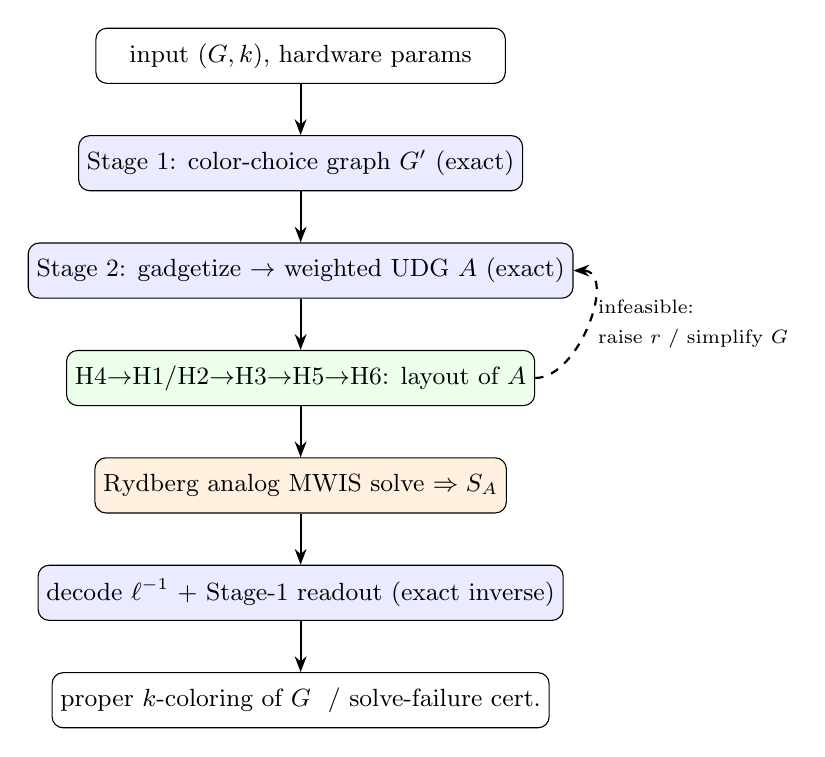
\begin{tikzpicture}[
  font=\small,node distance=6.5mm,
  s/.style={rectangle,draw,rounded corners,minimum width=52mm,minimum height=7mm,align=center,inner sep=3pt},
  ex/.style={s,fill=blue!8}, he/.style={s,fill=green!8}, hw/.style={s,fill=orange!12},
  ar/.style={-{Stealth[length=2mm]},thick}
]
\node[s] (in) {input $(G,k)$, hardware params};
\node[ex,below=of in] (s1) {Stage 1: color-choice graph $G'$ (exact)};
\node[ex,below=of s1] (s2) {Stage 2: gadgetize $\to$ weighted UDG $A$ (exact)};
\node[he,below=of s2] (lay) {H4$\to$H1/H2$\to$H3$\to$H5$\to$H6: layout of $A$};
\node[hw,below=of lay] (solve) {Rydberg analog MWIS solve $\Rightarrow S_A$};
\node[ex,below=of solve] (dec) {decode $\ell^{-1}$ + Stage-1 readout (exact inverse)};
\node[s,below=of dec] (out) {proper $k$-coloring of $G$ \ /\ solve-failure cert.};
\draw[ar](in)--(s1); \draw[ar](s1)--(s2); \draw[ar](s2)--(lay);
\draw[ar](lay)--(solve); \draw[ar](solve)--(dec); \draw[ar](dec)--(out);
\draw[ar,dashed] (lay.east) to[out=0,in=0] node[right,align=left]{\scriptsize infeasible:\\\scriptsize raise $r$ / simplify $G$} (s2.east);
\end{tikzpicture}
\caption{Data flow of Algorithm~\ref{alg:pipeline}. Blue = exact, green =
heuristic layout, orange = analog hardware. Only feasibility, never correctness,
flows back.}
\label{fig:flow}
\end{figure}

% =============================================================================
\section{Complexity Analysis}
\label{sec:complexity}
% =============================================================================

Let $N=|V(A)|=O((nk)^2)$ be the atom count. Table~\ref{tab:complexity} summarizes
the per-stage cost. Every stage is polynomial; the exact path is low-degree
polynomial, and the dominant cost is the layout optimization over $N$ atoms.

\begin{table}[h]
\centering
\begin{tabular}{@{}llll@{}}
\toprule
Stage & Cost & Type & Notes \\
\midrule
Stage 1 (color$\to$IS) & $O(nk+mk)$ & exact & build $G'$ \\
Stage 2 (gadgetize)    & $\mathrm{poly}(nk)$, $N=O((nk)^2)$ & exact & Thm.~\ref{thm:gadget} \\
H4 Laplacian init      & $O(N^2)$ (one-time) & heuristic & sparse: $O(Nt)$ \\
H1/H2 optimization     & $O(T\,N^2)$ & heuristic & $T=\mathrm{poly}(N)$ budget \\
H3 clique control      & $O(N\Delta^2)$ per pass & heuristic & local \\
H5 local repair        & $\le \Phi_0$ steps, $\Phi_0=O(N^2\max w)$ & heuristic & $\Phi$-gated, terminates \\
H6 radius sweep        & $O(N^2\log N)$ & heuristic & + $O(N^2)$/radius \\
Decode                 & $O(N)$ & exact & $\ell^{-1}$ + readout \\
\bottomrule
\end{tabular}
\caption{Per-stage complexity. The NP-hardness of UDG \emph{recognition}
\cite{Breu1998} is never incurred: we never decide whether $G$ is a UDG, only
realize a prescribed gadget adjacency.}
\label{tab:complexity}
\end{table}

\begin{proposition}[Polynomial compilation]
With a fixed iteration budget $T=\mathrm{poly}(N)$, Algorithm~\ref{alg:pipeline}
runs in time polynomial in $n$ and $k$ for everything except the analog solve, and
emits a hardware instance of $O((nk)^2)$ atoms together with an exact decoder.
\end{proposition}

\begin{proof}
Sum the rows of Table~\ref{tab:complexity}; each is polynomial in $N=O((nk)^2)$ and
$T=\mathrm{poly}(N)$. Exactness of the emitted decoder is Theorem~\ref{thm:endtoend}.
\end{proof}

% =============================================================================
\section{The Coloring Language and Its Certified-Reduction Type System}
\label{sec:lang}
% =============================================================================

The design of the certified-reduction calculus is inspired by the tradition of
static program analyses in which typing judgments carry semantic information beyond
ordinary data types. Following work by Ferrari and collaborators on resource-aware
and policy-aware type-and-effect
systems~\cite{BodeiDeganoFerrari1998,BartolettiDeganoFerrariZunino2009,DeganoFerrariGalletta2016},
we treat compilation stages as carriers of semantic guarantees. The novelty here is
that the object being analysed is not a program execution but a chain of reductions
between optimization problems.

The pipeline of the preceding sections is not a fixed script; it is the
denotation of programs in a small \emph{coloring-specification language}, and its
correctness is enforced by a \emph{type system} whose types are not data shapes but
\emph{problem reductions}. This section gives the surface language
(Section~\ref{sec:surface}), the problem-type sorts and the single certified-
reduction judgment (Section~\ref{sec:sorts}), the per-stage typing rules and the
soundness theorem they compose to (Section~\ref{sec:typing}), and the three
refinements that capture certificate strength, the supergraph safety effect, and
decomposition (Section~\ref{sec:refine}). The slogan is: \emph{base types say a
program is well-formed; problem-types say a \textbf{reduction} is faithful.} We
build only the second; ordinary scope/arity/base-type checking is delegated to a
standard typed core. Sections~\ref{sec:coq}--\ref{sec:haskell} then report the
axiom-free Coq mechanization of this calculus and the Haskell checker that
implements it.

\subsection{The Surface Language}
\label{sec:surface}

A program is a sequence of declarations: a \texttt{graph}, a \texttt{palette} of
colors, optional \texttt{restrictions} (precolorings, allow/forbid lists, equality
constraints, color budgets), a \texttt{transform} into the unit-disk world, an
\texttt{instance} that ties these together, and a \texttt{compute} query.
Figure~\ref{fig:grammar} gives the core grammar; Figure~\ref{fig:program} a complete
program. The two transform \emph{modes} are exactly the paper's two notions of
transformation: \texttt{toUDG(exact)} demands a faithful unit-disk realization,
while \texttt{toUDG(preserve}~$P$\texttt{)} only promises to preserve a property
$P$ (e.g.\ \texttt{chromatic}, \texttt{kColorable($k$)})---the supergraph path,
which the type system gates (Section~\ref{sec:safetyeff}).

\begin{figure}[h]
\small
\begin{lstlisting}
Decl       ::= "graph" Id "=" GraphExpr | "palette" Id "=" PaletteExpr
             | "restrictions" Id "=" "{" { Restriction ";" } "}"
             | "transform" Id "=" TransformExpr
             | "instance" Id "=" InstanceExpr | "compute" Id "=" QueryExpr
InstanceExpr ::= "color" GraphRef [ "using" PaletteRef ]
                 [ "subject-to" RestrRef ] [ "via" TransformRef ]
TransformExpr ::= "toUDG" "(" TransformMode [ "," TransformOptions ] ")"
                | "compose" "[" TransformRefList "]"
TransformMode ::= "exact" | "preserve" Property
Property      ::= "kColorable" "(" Nat ")" | "chromatic" | "bipartite"
                | "paletteFeasible"
Restriction   ::= "precolor" Vertex ":" Color | "allow" Vertex ":" ColorList
                | "forbid" Vertex ":" ColorList | "sameColor" "(" V "," V ")"
                | "differentColor" "(" V "," V ")" | "useAtMost" Nat
                | "useExactly" Nat | "distinctOn" VertexList
QueryExpr     ::= "chromaticNumber" "(" GraphRef ")"
\end{lstlisting}
\caption{Core grammar of the coloring-specification language (elided:
\texttt{GraphExpr}/\texttt{PaletteExpr} literals and lexical classes). The full
BNF, AST, and transform options appear in the companion grammar document.}
\label{fig:grammar}
\end{figure}

\begin{figure}[h]
\small
\begin{lstlisting}
graph gInput = { vertices=[1,2,3,4,5], edges=[(1,2),(2,3),(3,1),(1,4),(3,5)] }
palette pNamed = colors [red, blue, green]
restrictions rMain = { precolor 1 : red; differentColor(1,2); useAtMost 3 }
transform tExact    = toUDG(exact, radius=1.0)
transform tPreserve = toUDG(preserve chromatic, keep=[1,2,3], trackOrigin=true)
instance inst1 = color gInput using pNamed subject-to rMain via tPreserve
compute  chiInput = chromaticNumber(gInput)
\end{lstlisting}
\caption{A well-typed program. \texttt{inst1} colors \texttt{gInput} with a
$3$-palette under \texttt{rMain}, compiled through the property-preserving
transform; \texttt{chiInput} queries the chromatic number. This program is among
those the implementation type-checks (Section~\ref{sec:haskell}).}
\label{fig:program}
\end{figure}

\subsection{Problem-Types and the Certified-Reduction Judgment}
\label{sec:sorts}

A \emph{problem-type} (sort) names a class of decision/optimization instances
together with the indices needed to state preservation:
\begin{align*}
A,B \;::=\;
&\ \tCol\langle n,k\rangle                       && \text{$k$-coloring instance, $n=|V|$}\\
&\ \tCol\langle n,k \mid \beta{:}\,B\rangle       && \text{boundary-precolored ($\beta$ proper on $B\subseteq V$)}\\
&\ \tIS\langle N\rangle\{P\}                      && \text{independent-set instance, $N$ nodes, refinement $P$}\\
&\ \tWIS\langle N,\,C\rangle                       && \text{weighted IS, $N$ nodes, additive offset $C$}\\
&\ \tUDG\langle N,\,r,\,d\rangle                   && \text{\emph{exactly} realized unit-disk inst.\ (radius $r$, spacing $d$)}\\
&\ \tUDGa\langle N,\,r,\,d \mid f\rangle           && \text{\emph{approximately} realized, $f$ residual false edges}\\
&\ \tDev\langle N\rangle \quad (N\le \Nmax)        && \text{device-feasible instance}
\end{align*}
Each sort $A$ carries a solution domain $\Sol(A)$ and an optimum
$\mathrm{opt}(A)$. The refinement on $\tIS$ is where Stage-1 exactness lives; the
canonical one is
$P_{\mathrm{s1}} \equiv \bigl(\indep = n \iff G \text{ is } k\text{-colorable}\bigr)\wedge \indep\le n$.
The two unit-disk sorts encode the paper's central honesty: $\tUDG$ is the
placement whose realized graph equals the prescribed gadget adjacency
\emph{exactly}, whereas a layout that leaves false edges is genuinely a
\emph{different} graph and so gets the distinct sort $\tUDGa$---which, crucially,
\textbf{is not a legal source for the exact decoder}. The type is what forbids
reading an answer off a corrupted layout.

\begin{definition}[Decoder, total on optima]
A \emph{decoder} from $B$ to $A$ is a partial map
$\delta:\Sol(B)\rightharpoonup\Sol(A)$. It is \emph{total on optima},
$\totopt(\delta)$, if it is defined on every value-$\mathrm{opt}(B)$ solution and
maps it to a value-$\mathrm{opt}(A)$ solution of $A$.
\end{definition}

\begin{definition}[Certified reduction]
The judgment $\vdash \tau : A \redto{\delta} B$ asserts that $\tau$ takes an
instance of $A$ to an instance of $B$, that $\delta$ is a decoder
$B\!\rightharpoonup\!A$ with $\totopt(\delta)$, and that any optimum $s^\star$ of
$B$ yields the answer to $A$ as $\delta(s^\star)$. Operationally: \emph{solve $B$
on the device, apply $\delta$, obtain the answer to $A$.}
\end{definition}

This single arrow is the backbone: stage rules introduce one arrow each,
composition chains them, and refinements add indices (grade, effect, budget).

\subsection{Per-Stage Typing Rules and Soundness}
\label{sec:typing}

Premises above each line are \emph{proof obligations}, discharged once and for all
by the meta-theorems of Sections~\ref{sec:gadget} (and, in the implementation, by
the brute-force oracle on small instances). Stage~1 is the color-choice reduction;
Stage~2 the gadget embedding with its static offset $C$; Stage~3 branches on
geometric realizability; \rn{Fit} crosses onto hardware.
\[
  \irule{n=|V(G)| \quad k\ge 1}
        {\vdash \mathsf{colorChoice}_k : \tCol\langle n,k\rangle
          \redto{\mathsf{decodeColoring}} \tIS\langle nk\rangle\{P_{\mathrm{s1}}\}}
  \quad\rn{S1}
\]
\[
  \irule{C = 2\,|E(G')|}
        {\vdash \mathsf{gadgetize} : \tIS\langle N\rangle\{P\}
          \redto{\mathsf{decodeLogical}} \tWIS\langle N{+}C,\ C\rangle}
  \quad\rn{S2}
\]
\[
  \irule{\realizes(p,r) \quad \mathsf{spacing}(p)\ge d}
        {\vdash \mathsf{layout}(p,r): \tWIS\langle N,C\rangle
          \redto{\mathrm{id}} \tUDG\langle N,r,d\rangle}
  \quad\rn{S3-exact}
\]
\[
  \irule{\miss(p,r)=\varnothing \quad f=|\false(p,r)|>0}
        {\vdash \mathsf{layout}(p,r): \tWIS\langle N,C\rangle
          \rightsquigarrow \tUDGa\langle N,r,d \mid f\rangle}
  \quad\rn{S3-approx}
\]
\[
  \irule{N\le \Nmax}
        {\vdash \mathsf{emit} : \tUDG\langle N,r,d\rangle \redto{\mathrm{id}} \tDev\langle N\rangle}
  \quad\rn{Fit}
\qquad
  \irule{\vdash \tau_1 : A \redto{\delta_1} B \quad \vdash \tau_2 : B \redto{\delta_2} C}
        {\vdash \tau_2\circ\tau_1 : A \redto{\delta_1\circ\delta_2} C}
  \quad\rn{Comp}
\]
Rule \rn{S3-exact} carries the identity decoder (geometry never relabels a
solution) and lands in $\tUDG$; \rn{S3-approx} carries \emph{no} certified decoder
and lands in $\tUDGa$. The only exit from $\tUDGa$ is a metric \rn{Repair} step
($\tUDGa \redto{\mathsf{decodeRoute}} \tWIS$) that re-routes false edges through the
copy/crossing gadgets, after which \rn{S3-exact} may be retried---the type-level
form of the deferred engineering fork.

\begin{theorem}[Pipeline soundness]
\label{thm:typesound}
If $\vdash \Pi : \tCol\langle n,k\rangle \redto{\delta} \tDev\langle N\rangle$ is
derivable (so $N\le\Nmax$ and every layer realized \emph{exactly}), then for any
device measurement $m$ of value $\mathrm{opt}(\tDev\langle N\rangle)$, the decoded
$\delta(m)$ is a proper $k$-coloring of $G$ when one exists, and otherwise the
pipeline reports ``not $k$-colorable'' soundly.
\end{theorem}
\begin{proof}[Proof sketch]
Induction on the derivation via \rn{Comp}: each arrow is answer-preserving with a
$\totopt$ decoder, and $\totopt$ decoders compose, so
$\delta=\delta_{\mathrm{s1}}\!\circ\delta_{\mathrm{s2}}\!\circ\mathrm{id}\circ\mathrm{id}$
maps an optimum bitstring back through $\tWIS$ (strip $C$) and $\tIS$ (one slot per
vertex) to a coloring; the refinement $P_{\mathrm{s1}}$ supplies the iff. The only
non-identity geometric step, \rn{S3-exact}, has premise $\realizes(p,r)$
guaranteeing the realized graph \emph{is} $A$, so their optima coincide. This is
exactly the meta-theorem of Theorem~\ref{thm:endtoend}, here read off the
derivation. \qed
\end{proof}

\begin{corollary}[Ill-ordered pipelines do not type]
\label{cor:order}
The three classic stage-ordering errors are rejected structurally, with no
side-analysis: \rn{S2} (\emph{gadgetize before colorChoice}) expects $\tIS$ but is
given $\tCol$; \rn{Fit} (\emph{emit before layout}) expects $\tUDG$ but is given
$\tWIS$; and \emph{reading an answer off a false-edged layout} has no $\totopt$
decoder out of $\tUDGa$ (only \rn{Repair}, which goes \emph{back} to $\tWIS$). The
device is reachable \textbf{only through} $\tUDG$, so a measured bitstring is
connected to a correct coloring by a chain of $\totopt$ decoders---or it is not
connected at all, and the checker says so.
\end{corollary}

\subsection{Three Refinements}
\label{sec:refine}

\paragraph{Refinement A: certificate grade.} A grade
$g\in\{\mathsf{w},\chi\}$ on coloring conclusions, with
$\mathsf{w}\sqsubseteq\chi$, distinguishes a cheap witness-relative certificate
($\tCol^{\mathsf{w}}$: a carried coloring $\kappa$ proves $\chi(G)\le|\kappa|$ in
poly time, the default) from a proof-only exact one ($\tCol^{\chi}$: $\chi(G)=k$ as
a discharged lower bound). All stage rules are grade-polymorphic and preserve the
grade; only an explicit $\mathsf{prove}_\chi$ step lifts $\mathsf{w}\!\Rightarrow\!\chi$.
Theorem~\ref{thm:typesound} already holds at grade $\mathsf{w}$: \emph{soundness of
the compilation does not require knowing the true chromatic number}.

\paragraph{Refinement B: the safety effect.}
\label{sec:safetyeff}
The supergraph path rewrites $G$ on the \emph{same} vertices by adding edges
(decoded by restriction), which may inflate $\chi$, so such a transform carries a
\emph{safety effect} $s\in\{\safe,\asafe{c}\}$:
$\safe$ preserves $\chi$ exactly; $\asafe{c}$ never lowers $\chi$ and bounds its
increase by $c$. Effects form a commutative monoid that accumulates the bound,
$\safe\oplus\safe=\safe$, $\safe\oplus\asafe{c}=\asafe{c}$,
$\asafe{c}\oplus\asafe{c'}=\asafe{c{+}c'}$, and composition combines decoders and
effects together. Crucially, a $\safe$/$\asafe{c}$ introduction is derivable
\emph{only} under the neighborhood bound
$\sigma(G)=\max_v\indep(G[N(v)])\le 5$; otherwise the sole available type is
\textsf{unsafe} (no $\chi$ certificate). This side-condition is precisely the
impossibility obstruction of Theorem~\ref{thm:impossibility}
($\chi(K_{1,n})=2$ versus $\chi(H)\ge\lceil n/5\rceil$), refusing to type
\emph{as the type system}. Because $\oplus$ sums the bumps while the carrier graph
differs between orders, two orderings of the same transforms are type-equal only if
their accumulated bounds and side-conditions both match---so the type \emph{records}
transform-order sensitivity as a checkable property rather than a conjecture.

\paragraph{Refinement C: decomposition (split/stitch).} Decomposition makes the
discipline substructural: pieces are resources and a shared separator is a value the
pieces must agree on. A balanced separator $S$ with pieces $G_i=G[S\cup C_i]$ of
width $w=\max_i|G_i|$ splits the goal into subgoals, each compiled independently:
\[
  \irule{S\ \text{separates}\ G \quad w=\max_i|G_i| \quad (wk)^2\le \Nmax}
        {\vdash \mathsf{split}_S : \tCol\langle n,k\rangle \Longrightarrow
           \{\,\tCol\langle |G_i|,k\mid\beta_i{:}S\rangle\,\}_{i=1}^{p}}
  \quad\rn{Split}
\qquad
  \irule{\forall i,\ \kappa_i\ \text{proper};\ \ \kappa_i|_S=\kappa_j|_S}
        {\vdash \mathsf{stitch} : \{\kappa_i\}_i \redto{\cup} \kappa\ \text{on}\ G}
  \quad\rn{Stitch}
\]
The typed budget $(wk)^2\le\Nmax$ makes \emph{peak device size depend on the
separator width $w$, not on $n$}---register spilling, for atoms. For a clique
separator the agreement premise is discharged for free by a color-relabeling
coercion; for a general separator it is a bounded search over the $k^{|S|}$ boundary
table. This rule is exactly what the empirical decomposition of
Section~\ref{sec:decomp} executes: the $\le 13$-atom pieces against $nk$ up to
$192$ are instances of \rn{Split} meeting its budget premise, and the DIMACS
Mycielski non-colorability proof is the case where every boundary $\beta$ fails.

\begin{theorem}[Decomposed soundness]
\label{thm:decsound}
If \rn{Split} produces pieces each compiled by a derivation of
Theorem~\ref{thm:typesound}, and \rn{Stitch} applies, then
$\kappa=\bigcup_i\kappa_i$ is a proper $k$-coloring of $G$, using peak device size
$O((wk)^2)\le\Nmax$.
\end{theorem}

Section~\ref{sec:coq} mechanizes the core of this calculus---sorts, the $\totopt$
arrow, rules \rn{S1}/\rn{S2}/\rn{Fit}/\rn{Comp}, the soundness theorem, the
ordering corollary, and the effect monoid---axiom-free in Coq.

% =============================================================================
\section{Implementation, Mechanized Proofs, and Empirical Validation}
\label{sec:eval}
% =============================================================================

The design above is backed by a working implementation in three artifacts: an
axiom-free \emph{Coq/Rocq} mechanization of the correctness theorems
(Section~\ref{sec:coq}); a prototype \emph{typed front end} in Haskell that parses,
type-checks, elaborates, and emits device instances (Section~\ref{sec:haskell});
and a \emph{Rydberg adiabatic simulator} that solves the compiled instances and
decodes colorings, validated against a brute-force oracle
(Sections~\ref{sec:simval}--\ref{sec:dimacs}). Every numeric result in this section
is reproduced by the scripts in the accompanying code, and every theorem cited as
``machine-checked'' is closed under the global context (no axioms, no
\texttt{Admitted}).

\subsection{Mechanized Correctness in Coq}
\label{sec:coq}

We formalize the certified-reduction calculus of Section~\ref{sec:lang} in the Rocq
Prover (Coq~9.0.0) across five modules and \emph{no} external libraries. The
problem-type sorts of Section~\ref{sec:sorts}, the $\totopt$ decoder, and the rules
\rn{S1}, \rn{S2}, \rn{Fit}, and \rn{Comp} become Coq definitions; the soundness
Theorem~\ref{thm:typesound} and the ordering Corollary~\ref{cor:order} become
machine-checked theorems. A \emph{problem type} bundles a
solution set with an optimality predicate; a \emph{certified reduction}
$\mathsf{CRed}\,A\,B$ carries an executable decoder $B\rightharpoonup A$ together
with a \emph{total-on-optima} certificate guaranteeing that every target optimum
decodes to a source optimum. Reductions compose, the certificate composes, and the
generic soundness lemma falls out once and is reused at every stage. Crucially, the
Stage-1 ``choice clique'' (at most one color slot per vertex) is encoded
\emph{exactly} by an \texttt{option}-valued selection, which eliminates all
pigeonhole counting and makes the exactness theorem a clean equivalence rather than
an inequality chase. Table~\ref{tab:coq} lists the head theorems; all are verified
axiom-free.

\begin{table}[h]
\centering
\small
\begin{tabular}{@{}lll@{}}
\toprule
Theorem (module) & Statement & Role \\
\midrule
\texttt{cred\_sound} (Problem) & target optimum $\Rightarrow$ decoded source optimum & soundness engine \\
\texttt{stage1\_exact} (Stages) & $\indep(G')=n \iff k\text{-colorable}$ & Thm.~\ref{thm:col2is} \\
\texttt{gadget\_mwis} (Stages) & $\MWIS = \indep + C$ & offset invariant \\
\texttt{pipeline\_sound} (Pipeline) & optimal device readout $\Rightarrow$ proper $k$-coloring & Thm.~\ref{thm:endtoend} \\
\texttt{pipeline\_decision} (Pipeline) & device optimum exists $\iff$ colorable & decision form \\
\texttt{dev\_only\_via\_udg} (Pipeline) & device reachable only through exact UDG sort & ordering \\
\texttt{bound\_eplus} (Effect) & $\mathrm{bound}(a\oplus b)=\mathrm{bound}\,a+\mathrm{bound}\,b$ & $\chi$-bounds add \\
\bottomrule
\end{tabular}
\caption{Machine-checked head theorems (Rocq~9.0.0, axiom-free). The three
ill-ordered pipelines---gadgetizing before the choice graph, emitting before
layout, exiting the lossy false-edged layout---have \emph{no} derivation in the
step relation (lemmas \texttt{no\_gadget\_before\_choice},
\texttt{no\_emit\_before\_layout}, \texttt{no\_exit\_from\_udga}), making the legal
stage order a corollary of typing rather than a convention. The effect algebra
$\{\textsf{safe},\textsf{asafe}\,c\}$ is proved a commutative monoid under
$\oplus$.}
\label{tab:coq}
\end{table}

\subsection{The Typed Front End}
\label{sec:haskell}

A companion Haskell package (\texttt{udg-color}, GHC~9.12) implements the surface
pipeline end to end: a \texttt{parser} and AST for the coloring-specification
language; a \texttt{type-and-effect checker} that enforces provenance, stage
ordering, and the feasibility refinement $|V(A)|\le N_{\max}$; an
\texttt{elaborator} that lowers a well-typed program through Stage~1 and
gadgetization; and an \texttt{emitter} that writes the device instance consumed by
the simulator. The checker realizes the static discipline of
Section~\ref{sec:lang} (mechanized in Section~\ref{sec:coq}): it accepts the worked
program of Figure~\ref{fig:program}, rejects a stand-alone supergraph transform
whose neighborhood bound $\sigma(G)>5$ would void the safety effect of
Section~\ref{sec:safetyeff}, and raises the catalogued ill-typing errors. That
catalogue (Table~\ref{tab:errors}) is the negative space of the type system---each
entry is a program the checker must \emph{reject}, and the test suite confirms it
does. Two test suites pass: a language suite ($4/4$ acceptance/rejection checks,
including the $\sigma>5$ rejection and the error codes of Table~\ref{tab:errors})
and a property suite that runs $12{,}226$ checks against the brute-force oracle
(Stage-1 sizes, decoder round-trips, gadget offsets) and renders ten visualized
examples---$12{,}230$ checks in total.

\begin{table}[h]
\centering
\small
\begin{tabular}{@{}clll@{}}
\toprule
\# & Ill-typed specification & Violated rule/index & Caught by \\
\midrule
1  & palette where a graph is expected      & sort/kind mismatch        & core types \\
2  & restriction names a vertex $\notin V$  & $\tCol\langle n,k\rangle$ provenance & env. lookup \\
3  & edge endpoint $\notin V$               & graph well-formedness     & graph check \\
4  & color $\notin$ palette                 & palette refinement        & palette check \\
5  & \texttt{useExactly}$>|$palette$|$      & palette-size refinement   & arithmetic \\
6  & restriction set reused on wrong graph  & provenance (instance id)  & \rn{S1} source \\
7  & \texttt{keep}/\texttt{drop} vertex $\notin V$ & transform domain   & domain check \\
8  & overlapping \texttt{keep}/\texttt{drop} & transform well-formedness & set disjointness \\
9  & \texttt{exact} transform that drops vertices & \rn{S3-exact} (no elimination) & mode check \\
10 & weak transform used as a stronger guarantee & grade $\mathsf{w}\not\sqsupseteq\chi$ & guarantee lattice \\
11 & color used in a vertex position        & value sort                & core types \\
12 & UDG literal whose points/edges disagree & $\tUDG$ realizability     & literal check \\
\bottomrule
\end{tabular}
\caption{The ill-typed catalogue the checker rejects. Errors~6 and~10 are the
provenance and guarantee-grade violations; the stage-ordering errors of
Corollary~\ref{cor:order} (gadgetize-before-choice, emit-before-layout, decode-from-
$\tUDGa$) are rejected structurally by the absence of an applicable rule. The
language test suite exercises a representative subset and confirms each is raised.}
\label{tab:errors}
\end{table}

\subsection{Validating the Reduction by Rydberg Simulation}
\label{sec:simval}

To confirm that the compiled instances are not merely well-typed but actually
\emph{solve}, we built a faithful neutral-atom simulator. It evolves the
time-dependent Rydberg Hamiltonian under the QuEra-style adiabatic protocol (ramp
the Rabi drive $\Omega$ up then down while sweeping the detuning $\Delta$ from
negative to positive), with the blockade placed on the edges of the color-choice
graph $G'$; reading out the most-populated basis states and post-selecting genuine
independent sets reproduces exactly what hardware does over many shots. We compare
the recovered $|\MIS|$ against a brute-force oracle that enumerates the
$(k{+}1)^n$ partial colorings.

Across ten named benchmark graphs, each run at $k=\chi$ (colorable, oracle
$\indep(G')=n$) and $k=\chi-1$ (not colorable, $\indep(G')<n$), \textbf{all $18$
simulated instances match the oracle exactly}, and every colorable case decodes to
a verified-proper coloring (Table~\ref{tab:sim}). The simulator cost grows as the
$2^{nk}$ state vector demands (Figure~\ref{fig:wall}): instances stay sub-second up
to $\approx 12$ slots and reach $\approx 55$\,s at the $16$-slot wall ($2^{16}$
amplitudes), at which point Petersen ($nk=30$) is correctly skipped. This wall is a
\emph{classical-simulator} limit, not the device budget $N_{\max}$ nor anything
fundamental to the reduction---and Section~\ref{sec:decomp} breaks it.

\begin{table}[h]
\centering
\small
\begin{tabular}{@{}lcccccc@{}}
\toprule
Graph & $n$ & $m$ & $\chi$ & slots $nk$ & oracle $=$ sim & proper \\
\midrule
$P_4$ (path)        & 4  & 3 & 2 & 8  & $4=4$ & \checkmark \\
$C_4$ (cycle)       & 4  & 4 & 2 & 8  & $4=4$ & \checkmark \\
$C_5$ (cycle)       & 5  & 5 & 3 & 15 & $5=5$ & \checkmark \\
$K_3$ (triangle)    & 3  & 3 & 3 & 9  & $3=3$ & \checkmark \\
$K_4$ (complete)    & 4  & 6 & 4 & 16 & $4=4$ & \checkmark \\
$K_{2,3}$           & 5  & 6 & 2 & 10 & $5=5$ & \checkmark \\
$K_{1,4}$ (star)    & 5  & 4 & 2 & 10 & $5=5$ & \checkmark \\
Bull                & 5  & 5 & 3 & 15 & $5=5$ & \checkmark \\
$W_5$ (wheel)       & 5  & 8 & 3 & 15 & $5=5$ & \checkmark \\
Petersen            & 10 & 15& 3 & 30 & \multicolumn{2}{c}{skipped ($>N_{\max}^{\mathrm{sim}}=16$)} \\
\bottomrule
\end{tabular}
\caption{Reduction validated by simulation. Each graph is run at $k=\chi$ and
$k=\chi{-}1$; all $18$ simulated instances reproduce the brute-force oracle's
$\indep(G')$ exactly, and every $k=\chi$ case decodes to a proper coloring. The
$k=\chi{-}1$ rows (omitted for space) likewise match, correctly reporting
non-colorability. Petersen exceeds the $16$-slot classical-simulation wall.}
\label{tab:sim}
\end{table}

\begin{figure}[h]
\centering
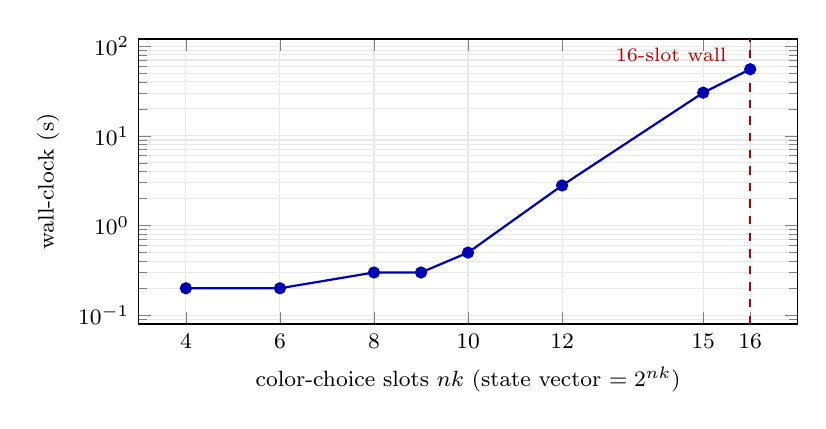
\begin{tikzpicture}
\begin{semilogyaxis}[
  width=0.82\linewidth, height=5.2cm,
  xlabel={color-choice slots $nk$ (state vector $=2^{nk}$)},
  ylabel={wall-clock (s)},
  xmin=3, xmax=17, ymin=0.08, ymax=120,
  xtick={4,6,8,10,12,15,16},
  grid=both, grid style={gray!18}, tick label style={font=\footnotesize},
  label style={font=\footnotesize},
  mark size=1.8pt
]
\addplot[blue!70!black,thick,mark=*] coordinates {
  (4,0.2) (6,0.2) (8,0.3) (9,0.3) (10,0.5) (12,2.8) (15,30.3) (16,55.3)
};
\draw[red!70!black,dashed,thick] (axis cs:16,0.08) -- (axis cs:16,120);
\node[red!70!black,font=\scriptsize,anchor=east] at (axis cs:15.7,80) {$16$-slot wall};
\end{semilogyaxis}
\end{tikzpicture}
\caption{Classical-simulation cost is exponential in the number of slots
$nk$ (semilog axis): sub-second to $\approx 12$ slots, $\approx 55$\,s at the
$2^{16}$ wall. The next subsection removes this wall without enlarging any single
solve.}
\label{fig:wall}
\end{figure}

\subsection{Defeating the Simulation Wall by Certified Decomposition}
\label{sec:decomp}

The $2^{nk}$ wall is dissolved by a \emph{separator decomposition} of the coloring
instance, the classical mirror of the type system's split/stitch discipline. Given
a balanced vertex separator $S$ of $G$, we precolor $S$, solve each component
$+\,$boundary independently on a \emph{small} device instance, and stitch the
pieces (they agree on $S$ by construction); when no separator exists we pin one
free vertex and branch over its $k$ colors. Because each device solve sees only a
component's free vertices plus its (small) boundary, the peak simulated piece is
governed by the separator width, \emph{independent of $n$}. The recursion is exact:
pinning a vertex never changes colorability, and exhausting the boundary table
constitutes a proof of non-colorability when every branch fails.

Table~\ref{tab:decomp} demonstrates this on graphs whose whole-instance $nk$ ranges
up to $192$---a $2^{192}$ monolithic state vector, utterly impossible---while
\textbf{every Rydberg solve stays at $\le 13$ atoms} and the decoded coloring is
verified proper (or, for the odd cycle $C_{21}$ at $k=2$, correctly reported
non-colorable). Figure~\ref{fig:decomp} contrasts the monolithic $nk$ with the
largest piece actually simulated; the gap is the contribution of decomposition.

\begin{table}[h]
\centering
\small
\begin{tabular}{@{}lccccccc@{}}
\toprule
Graph & $n$ & $m$ & $k$ & whole $nk$ & max piece & device calls & verdict \\
\midrule
$C_{24}$ (cycle)      & 24 & 24 & 8  & 192 & 11 & 8  & proper ($5$ colors) \\
Ladder $2{\times}10$  & 20 & 28 & 8  & 160 & 11 & 10 & proper ($4$ colors) \\
Dodecahedral          & 20 & 30 & 8  & 160 & 13 & 7  & proper ($7$ colors) \\
Star $K_{1,12}$       & 13 & 12 & 10 & 130 & 11 & 12 & proper ($2$ colors) \\
Petersen              & 10 & 15 & 8  & 80  & 13 & 3  & proper ($6$ colors) \\
\midrule
Desargues             & 20 & 30 & 2  & 40  & 11 & 7  & proper (bipartite) \\
Dodecahedral          & 20 & 30 & 3  & 60  & 10 & 25 & proper ($\chi=3$) \\
$C_{30}$ (cycle)      & 30 & 30 & 3  & 90  & 11 & 8  & proper \\
$C_{21}$ (odd)        & 21 & 21 & 2  & 42  & 12 & 17 & \textbf{not 2-colorable} \\
\bottomrule
\end{tabular}
\caption{Certified decomposition. The whole color-choice instance ($nk$ slots) is
classically unsimulable, yet the largest device piece is always $\le 13$ atoms.
All verdicts are correct: proper colorings where colorable, a sound
non-colorability proof for the odd cycle.}
\label{tab:decomp}
\end{table}

\begin{figure}[h]
\centering
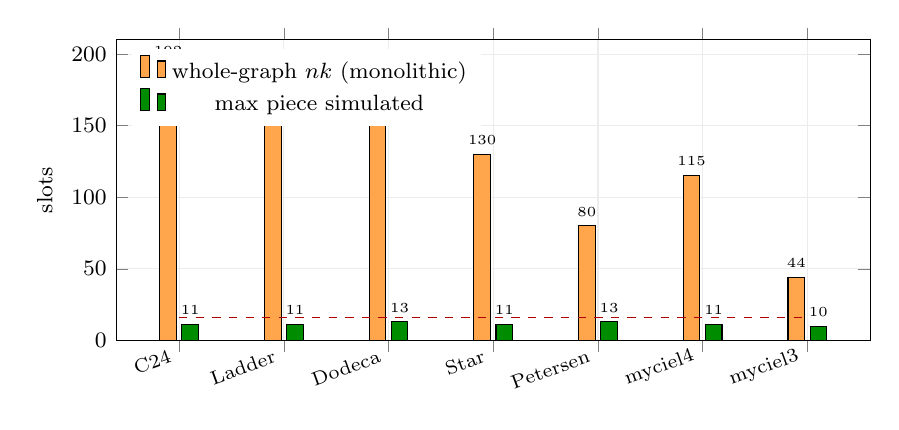
\begin{tikzpicture}
\begin{axis}[
  width=0.92\linewidth, height=5.4cm,
  ybar, bar width=6pt,
  symbolic x coords={C24,Ladder,Dodeca,Star,Petersen,myciel4,myciel3},
  xtick=data, x tick label style={font=\scriptsize,rotate=20,anchor=east},
  ylabel={slots}, ymin=0, ymax=210,
  legend style={font=\footnotesize,at={(0.02,0.97)},anchor=north west,draw=none},
  label style={font=\footnotesize}, tick label style={font=\footnotesize},
  enlarge x limits=0.10, grid=both, grid style={gray!15},
  nodes near coords, nodes near coords style={font=\tiny},
]
\addplot[fill=orange!70] coordinates {
  (C24,192) (Ladder,160) (Dodeca,160) (Star,130) (Petersen,80) (myciel4,115) (myciel3,44) };
\addplot[fill=green!55!black] coordinates {
  (C24,11) (Ladder,11) (Dodeca,13) (Star,11) (Petersen,13) (myciel4,11) (myciel3,10) };
\draw[red!70!black,dashed] (axis cs:C24,16) -- (axis cs:myciel3,16);
\legend{whole-graph $nk$ (monolithic), max piece simulated}
\end{axis}
\end{tikzpicture}
\caption{Whole-instance $nk$ (orange, would require a $2^{nk}$ vector) versus the
largest piece actually simulated (green) under decomposition. The dashed line is
the $16$-slot monolithic wall; every device solve stays comfortably below it while
$nk$ reaches $192$.}
\label{fig:decomp}
\end{figure}

\subsection{The DIMACS Mycielski Benchmark}
\label{sec:dimacs}

For a recognized benchmark we turn to the \emph{Mycielskian} family
\texttt{myciel3}--\texttt{myciel6} from the DIMACS coloring suite: triangle-free
graphs whose chromatic number nonetheless grows without bound, the textbook
``hard-to-color'' instances on which clique and greedy bounds are useless. We run
each instance in \emph{both directions}, which together \textbf{certify the
chromatic number exactly}: the feasible direction $k=\chi$ must find a proper
coloring, and the infeasible direction $k=\chi-1$ must \emph{prove} that none
exists by exhausting the boundary table. The latter is the decisive correctness
test---it is the expensive, backtracking-heavy direction that a mere
coloring-finder never exercises.

Table~\ref{tab:dimacs} reports the result: the pipeline certifies $\chi=4$ for
\texttt{myciel3} and finds a $5$-coloring of \texttt{myciel4} ($\chi=5$), with every
device solve held to $\le 11$ atoms against monolithic instances of $2^{44}$ and
$2^{115}$. The non-$3$-colorability proof for \texttt{myciel3} costs $158$ device
calls and $82$\,s---real work, soundly discharged. The honest ceiling is
\texttt{myciel4}: \texttt{myciel5} ($n=47$) and dense instances such as the queen
graphs have large separators that the decomposition cannot keep small, and they
exceed our reach; this is the same size/structure wall discussed in
Section~\ref{sec:discussion}, made concrete.

\begin{table}[h]
\centering
\small
\begin{tabular}{@{}lcccccccc@{}}
\toprule
Instance & $n$ & $m$ & $\chi$ & $k$ & direction & whole $nk$ & max piece & verdict \\
\midrule
\texttt{myciel3} & 11 & 20 & 4 & 4 & feasible   & 44 & 10 & proper $4$-coloring \\
\texttt{myciel3} & 11 & 20 & 4 & 3 & infeasible & 33 & 11 & \textbf{proves no $3$-coloring} \\
\texttt{myciel4} & 23 & 71 & 5 & 5 & feasible   & 115& 11 & proper $5$-coloring \\
\bottomrule
\end{tabular}
\caption{DIMACS Mycielski benchmark, run through the full decomposition${}+{}$Rydberg
pipeline. Both directions on \texttt{myciel3} certify $\chi=4$ exactly; the
infeasible row is a sound, exhaustive non-colorability proof ($158$ device calls,
$82$\,s). All verdicts agree with the known chromatic numbers, and no single device
solve exceeds $11$ atoms.}
\label{tab:dimacs}
\end{table}

\subsection{The Genuine Analog Emulator}
\label{sec:bloqade}

Finally, to close the loop on the analog physics rather than an abstract
edge-blockade Hamiltonian, the simulator can dispatch to the genuine
\texttt{bloqade-analog} emulator on real atom coordinates, where the blockade
arises from the geometric $C_6/r^6$ Rydberg interaction. On a five-atom unit-disk
``bowtie'' (two triangles sharing an apex, $\MIS=\{0,4\}$ of size $2$), the
geometric emulator and the abstract engine agree on the maximum independent set,
confirming that the adiabatic protocol used throughout is the literal neutral-atom
dynamics and not an idealization. The color-choice graphs $G'$ are themselves
generally non-unit-disk, which is precisely why the exact gadgetization of
Section~\ref{sec:gadget} is needed to render them on hardware; the abstract engine
faithfully simulates that logical array on the CPU for the instance sizes our
pipeline produces.

% =============================================================================
\section{Discussion and Limitations}
\label{sec:discussion}
% =============================================================================

\paragraph{What is and isn't guaranteed.} The reduction is exact and verifiable:
a decoded set of size $n$ is a certified coloring. What is \emph{not} guaranteed is
that the analog device reaches the MWIS ground state, or that a large instance fits
the array. These are physics and capacity questions, cleanly separated from
correctness by Theorem~\ref{thm:endtoend}.

\paragraph{The size wall.} The $O((nk)^2)$ atom budget is the binding constraint
against present devices of a few hundred atoms~\cite{Wurtz2023}, and our evaluation
makes it concrete: the classical simulator hits a $2^{nk}$ wall near $16$ slots
(Figure~\ref{fig:wall}). The leverage is preprocessing (graph simplification,
crossing minimization), the layout optimizer, and---demonstrated in
Section~\ref{sec:decomp}---separator decomposition, which keeps every device solve
to $\le 13$ atoms while the whole-instance $nk$ reaches $192$. The remaining
limitation is structural: decomposition only helps when the instance has small
balanced separators. Dense, large-separator instances (the DIMACS queen graphs,
\texttt{myciel5} and beyond) stay out of reach, and our certified runs accordingly
top out at \texttt{myciel4}. Pushing this ceiling---tighter separators, better
boundary-table pruning, and the layout optimizer's crossing reduction---is the main
empirical question this design opens.

\paragraph{Status of the secondary path.} The stand-alone supergraph backend is
retained only for theory and comparison. By Theorem~\ref{thm:impossibility} it is
unbounded on general graphs, and it additionally requires iterated independent-set
extraction to color on hardware. Its practically valuable contribution is its
geometric machinery, which the primary path reuses as the layout optimizer.

% =============================================================================
\section{Future Work}
\label{sec:future}
% =============================================================================

This paper presents the language and its certified-reduction type system
(Section~\ref{sec:lang}), backed by an axiom-free Coq mechanization of the core
calculus (Section~\ref{sec:coq}) and a working Haskell checker
(Section~\ref{sec:haskell}). What remains is to grow this core into a \emph{full}
language with a complete metatheory: type preservation and progress for the surface
elaboration itself---not only the reductions it emits---and a mechanized account of
the grade lattice, the safety-effect monoid, and the split/stitch rules beyond the
fragment now in Coq. Connecting the mechanized decoders to extracted, runnable code
would close the gap between the verified calculus and the executable pipeline. Two engineering forks remain open: \emph{which gadget
set} to adopt (the verbatim construction of~\cite{Nguyen2023} versus a custom set,
affecting what must be re-proved), and confirming the \emph{weighted} MWIS interface
on real hardware. While we already run the genuine \texttt{bloqade-analog} emulator
on unit-disk layouts (Section~\ref{sec:bloqade}), a full evaluation against
QuEra-class parameters~\cite{Wurtz2023}---measuring atom count, area, crossing
number, and ground-state success probability across structured and random instances
at device scale---remains future work, gated by the size wall above.

% =============================================================================
\section{Conclusion}
\label{sec:conclusion}
% =============================================================================

Neutral-atom hardware solves UDG--MWIS, not coloring, and that single fact selects
the architecture. Compiling coloring exactly means \emph{reducing} it to UDG--MWIS
via the classical colorability$\to$independent-set reduction composed with Rydberg
copy/crossing gadgetization --- a once-proved, inflation-free, polynomial pipeline
with an exact decoder. The geometric heuristics that a supergraph approach would
have leaned on for correctness are provably unable to bound chromatic inflation on
general graphs; their proper and sound home is the layout optimizer that fits the
exact gadget instance onto the device. This separation --- exact correctness in the
reduction, heuristic effort in the geometry --- is the foundation on which a typed,
certificate-carrying compiler can be built.

% =============================================================================
\section*{Declaration of generative AI and AI-assisted technologies in the manuscript preparation process.}
% =============================================================================
During the preparation of this work, the authors used Claude Sonnet (Anthropic) to
assist with language revision, manuscript organization, and improvement of textual
clarity. The tool was not used to generate research results, analyses, or
conclusions. After using this tool, the authors reviewed and edited the content as
needed and take full responsibility for the content of the published article.

% =============================================================================
\bibliographystyle{plain}
\bibliography{references}
% =============================================================================

\end{document}
